\documentclass[aps,prd,twocolumn,superscriptaddress,nofootinbib]{revtex4-2}

\usepackage{amsmath}
\usepackage{amssymb}
\usepackage{graphicx}
\usepackage{hyperref}
\usepackage{bm}

\graphicspath{{../results/}}

\newcommand{\Msun}{M_\odot}
\newcommand{\order}[1]{\mathcal{O}(#1)}

\begin{document}

\title{Quacky Normal Modes}

\author{Author One}
\affiliation{Department of Physics, University, City, Country}
\author{Author Two}
\affiliation{Department of Physics, University, City, Country}

\date{\today}

\begin{abstract}
We develop the general theory of oscillation modes, tidal deformability,
and gravitational wave signatures for non-spherical self-gravitating bodies,
using a rubber duck as the maximally asymmetric worked example.
Three main results emerge.
First, the complete breaking of spherical symmetry lifts the
$(2\ell+1)$-fold degeneracy of every quasinormal mode multiplet through a
mechanism we term \textit{gravitational Zeeman splitting}: the duck shape
deformation couples to the mode spectrum via Gaunt integrals and Wigner $3j$
symbols, producing a $5\times5$ perturbation matrix for the $\ell=2$
$f$-mode whose eigenvalues give five distinct frequencies with
$\Delta\omega/\omega\sim 0.3$.
Second, the tidal response is promoted from a scalar Love number $k_2$ to a
rank-4 Love tensor $\lambda_{ijkl}$ with up to 15 independent components,
and the celebrated I-Love-Q universality relations break down at
$\order{100\%}$ for duck-shaped objects.
Third, we confront the duck hypothesis with gravitational wave data across
the full frequency spectrum: the nanohertz stochastic background observed by
NANOGrav, EPTA, and PPTA is indistinguishable from a population of
inspiraling ducks, and stellar-mass duck mergers are consistent with
GW170817 tidal constraints.
We prove a population-level degeneracy theorem establishing that current
observations cannot exclude duck-shaped compact objects, and identify
next-generation QNM spectroscopy as the most promising path to a definitive
test.
\end{abstract}

\maketitle


%======================================================================
\section{Introduction}
\label{sec:intro}
%======================================================================

The spherical cow approximation (SCA) is among the most celebrated
simplifications in theoretical physics.
From Newtonian gravity to quantum chromodynamics, the replacement of a
complicated object with a sphere of equivalent mass has enabled generations
of physicists to obtain closed-form solutions where none would otherwise
exist.
The SCA is so deeply embedded in the culture of physics that it has become
both a pedagogical device and a punchline---a shorthand for the productive
audacity of theorists who privilege tractability over realism.

Recently, Lehmann~\cite{Lehmann2025} undertook a rigorous investigation of
the SCA's validity in the context of gravitational wave (GW) emission,
computing the full multipole structure of a Holstein dairy cow and evaluating
the resulting gravitational radiation.
The central result is devastating: the SCA fails catastrophically for GW
physics.
A perfect sphere, possessing only a monopole moment, radiates \textit{zero}
gravitational waves.
The cow's gravitational wave luminosity is entirely determined by its higher
multipole moments---the very features that the SCA discards.
This observation elevates the multipole structure of non-spherical bodies
from a curiosity to a matter of fundamental importance for gravitational
wave astronomy.

In the present work, we extend this program from the bovine to the anatine.
We develop the general theory of oscillation modes, tidal deformability, and
gravitational wave signatures for non-spherical self-gravitating bodies,
using a rubber duck as the worked example.
The resulting framework---which we term the theory of \textbf{quacky normal
modes} (QNMs)---reveals a rich phenomenology that is entirely absent in the
spherical limit.


\subsection{Why the Duck}
\label{sec:why_duck}

The choice of test geometry is not arbitrary.
While the cow is roughly ellipsoidal, retaining an approximate
$\mathbb{Z}_2$ symmetry about the sagittal plane and a near-axial symmetry
along the spine, the rubber duck breaks \textit{all} continuous symmetries
of $SO(3)$.
The duck possesses three geometrically distinct substructures---bill, neck,
and tail---each of which contributes independently to the spherical harmonic
content of the surface deformation.
In the language of the deformation spectrum,
\begin{equation}
R_{\mathrm{duck}}(\theta, \phi) = R_0 \left[ 1 + \sum_{\ell \geq 1}
\sum_{m=-\ell}^{\ell} \varepsilon_{\ell m}\, Y_\ell^m(\theta, \phi) \right],
\label{eq:Rduck}
\end{equation}
the duck exhibits significant power at all multipole orders $\ell \leq 8$,
with deformation amplitudes $|\varepsilon_{\ell m}| \sim 0.1$--$0.3$
extending to high $\ell$.
By contrast, the cow's deformation spectrum is dominated by $\ell = 2$
(the body ellipsoid) with rapid falloff at higher $\ell$.

The duck is therefore a \textbf{maximally non-spherical} test case: it
probes the regime where the SCA fails most dramatically, and where the full
machinery of degenerate perturbation theory is required to capture the
physics.


\subsection{Three Threads}
\label{sec:three_threads}

This paper develops three interconnected threads.

\textbf{Quacky normal modes and gravitational Zeeman splitting.}---The
normal modes of a spherical star are characterized by quantum numbers
$(n, \ell, m)$, where each $(n, \ell)$ multiplet is $(2\ell + 1)$-fold
degenerate.
The duck shape lifts this degeneracy completely: the deformation
$\varepsilon_{\ell' m'}$ couples to the mode spectrum through Gaunt
integrals involving Wigner $3j$ symbols, producing a perturbation matrix
\begin{equation}
V_{m_1 m_2}^{(n,\ell)} = -|R_{n\ell}'(R_0)|^2 R_0^3 \sum_{\ell', m'}
\varepsilon_{\ell' m'} \int_{S^2} Y_\ell^{m_1 *}\, Y_\ell^{m_2}\,
Y_{\ell'}^{m'}\, d\Omega
\label{eq:Vmatrix_intro}
\end{equation}
whose eigenvalues give the split frequencies.
We call this \textbf{gravitational Zeeman splitting}.
For the $\ell = 2$ $f$-mode, we predict a five-fold splitting with
$\Delta\omega / \omega \sim \order{\varepsilon} \sim 0.3$---a 30\% effect,
far larger than the $\sim 10^{-3}$ rotational splitting in millisecond
pulsars.

\textbf{Tidal Love numbers and the Love tensor.}---For a spherical body,
the tidal response is characterized by a single dimensionless number $k_2$.
For the duck, the response to an external tidal field $\mathcal{E}_{ij}$ is
described by a fourth-rank \textbf{Love tensor} $\lambda_{ijkl}$:
\begin{equation}
Q_{ij}^{\mathrm{induced}} = -\lambda_{ijkl}\, \mathcal{E}_{kl},
\label{eq:love_tensor_intro}
\end{equation}
a symmetric $5 \times 5$ matrix (in the space of traceless symmetric
tensors) with up to 15 independent components.
The celebrated I-Love-Q universality relations of Yagi and
Yunes~\cite{YagiYunes2013a, YagiYunes2013b}---which hold to
$\order{1\%}$ for all spherical neutron star equations of state---break
down catastrophically for the duck, with deviations of $\order{100\%}$ for
$\varepsilon \sim 0.3$.

\textbf{Observational indistinguishability.}---We confront the duck
hypothesis with current gravitational wave observations across the entire
frequency spectrum.
In the nanohertz band, a cosmological population of supermassive binary
ducks ($M \sim 10^6$--$10^9\, \Msun$) produces a stochastic gravitational
wave background with characteristic strain
\begin{equation}
h_c(f) = A_{\mathrm{duck}} \left( \frac{f}{f_{\mathrm{yr}}} \right)^{-2/3},
\label{eq:hc_duck}
\end{equation}
where $A_{\mathrm{duck}} = 2.4 \times 10^{-15}$---a value
indistinguishable from the signal reported by the NANOGrav 15-year
dataset~\cite{NANOGrav2023}, the European Pulsar Timing
Array~\cite{EPTA2023}, and the Parkes Pulsar Timing
Array~\cite{PPTA2023}.
We prove a \textbf{population-level degeneracy theorem}: for any SMBHB
population model consistent with current PTA data, there exists a binary
duck population with identical masses and merger rates that reproduces the
observed signal to arbitrary precision.

In the audio-frequency band, stellar-mass duck mergers
($M \sim 1$--$3\, \Msun$) produce ringdown waveforms with anomalous QNM
splitting.
The duck's anisotropic tidal deformability
$\tilde{\Lambda}_{\mathrm{duck}}$ lies within the broad constraints from
GW170817 ($\tilde{\Lambda} = 300^{+420}_{-230}$)~\cite{Abbott2017GW170817,
Abbott2018GW170817tidal}.
We conclude that current gravitational wave observations cannot exclude
the hypothesis that compact objects are duck-shaped.


\subsection{Paper Organization}
\label{sec:organization}

The paper is organized in three parts.

\textbf{Part~I: General Formalism} (Secs.~\ref{sec:geometry}--\ref{sec:binary})
develops the theoretical framework.
Section~\ref{sec:geometry} characterizes the duck geometry and its spherical
harmonic decomposition.
Section~\ref{sec:qnm} derives the quacky normal mode spectrum using
degenerate perturbation theory and the Hadamard domain perturbation formula.
Section~\ref{sec:love} develops the Love tensor formalism and establishes
the breakdown of I-Love-Q universality.
Section~\ref{sec:binary} constructs the post-Newtonian dynamics of binary
duck systems.

\textbf{Part~II: Numerical Simulations}
(Secs.~\ref{sec:fem}--\ref{sec:athenak}) validates and extends the analytic
results.
Section~\ref{sec:fem} presents finite-element solutions of the Helmholtz
eigenvalue problem on the duck domain.
Section~\ref{sec:athenak} describes full numerical relativity simulations
using AthenaK~\cite{Stone2024, Zhu2024, Fields2024}.

\textbf{Part~III: Observational Confrontation} (Sec.~\ref{sec:obs}) places
constraints on the duck hypothesis using gravitational wave data.

Section~\ref{sec:discussion} presents our conclusions.


\subsection{Notation and Conventions}
\label{sec:notation}

Throughout this paper we employ geometric units $G = c = 1$ unless otherwise
stated; factors of $G$ and $c$ are restored in expressions intended for
numerical evaluation.
The metric signature is $(-,+,+,+)$.
Spherical harmonics $Y_\ell^m(\theta, \phi)$ follow the Condon-Shortley
phase convention, with the normalization
\begin{equation}
\int_{S^2} Y_\ell^{m*}\, Y_{\ell'}^{m'}\, d\Omega = \delta_{\ell\ell'}\,
\delta_{mm'}.
\label{eq:SH_norm}
\end{equation}
Greek indices $\mu, \nu, \ldots$ run over spacetime coordinates
$\{0, 1, 2, 3\}$; Latin indices $i, j, \ldots$ run over spatial coordinates
$\{1, 2, 3\}$.
The compactness parameter is $C = M/R$ (in geometric units).
The dimensionless tidal deformability is
$\Lambda = (2/3)\, k_2\, C^{-5}$.
We use $\Msun$ for the solar mass and define
$f_{\mathrm{yr}} \equiv 1/\mathrm{yr} \approx 31.7\,\mathrm{nHz}$ as the
reference frequency for PTA analyses.


%======================================================================
\section{Duck Geometry and Multipole Characterization}
\label{sec:geometry}
%======================================================================

\subsection{The Duck Mesh}
\label{sec:duck_mesh}

We adopt as our fiducial \textit{Anas platyrhynchos} the DASSL rubber duck
mesh, comprising 4732 vertices and 9460 triangular faces.
The mesh is watertight and has been normalized to unit bounding-box scale.
The duck is oriented with the bill pointing along the negative $x$-axis, the
body extending in the $+x$ direction, and the vertical (head-to-belly) along
the $y$-axis.
Unlike the cow of Lehmann~\cite{Lehmann2025}, which is roughly ellipsoidal,
the duck possesses no continuous symmetry---the bill, neck, tail, and body
break all axial and planar symmetries, making it a maximally general test
case for non-spherical compact object physics.


\subsection{Volume Integrals and Multipole Moments}
\label{sec:multipoles}

We compute the duck's multipole moments using fan tetrahedralization from
the center of mass and Hammer-Stroud quadrature (4-point rule, exact for
degree-2 polynomials).

\textbf{Volume and center of mass.}
The volume is computed via the divergence theorem:
\begin{equation}
V = \frac{1}{6}\sum_{\text{faces}} \mathbf{v}_0 \cdot (\mathbf{v}_1 \times
\mathbf{v}_2).
\end{equation}

The equivalent sphere radius is
\begin{equation}
R_{\mathrm{eq}} = \left(\frac{3V}{4\pi}\right)^{1/3}.
\end{equation}

\textbf{Cartesian quadrupole tensor} (traceless, symmetric):
\begin{equation}
Q^C_{ij} = \int_{\mathcal{D}} \rho(\mathbf{x})(3x_i x_j - r^2
\delta_{ij})\,d^3\mathbf{x}.
\end{equation}

\textbf{Inertia tensor:}
\begin{equation}
I_{ij} = \int_{\mathcal{D}} \rho(\mathbf{x})(r^2 \delta_{ij} - x_i
x_j)\,d^3\mathbf{x}.
\end{equation}

These satisfy the cross-check relation
$Q^C_{ij} = \mathrm{Tr}(I)\,\delta_{ij} - 3I_{ij}$.

\textbf{Spherical multipole moments} up to $\ell = 10$:
\begin{equation}
Q_\ell^m = \int_{\mathcal{D}} \rho(\mathbf{x})\,\|\mathbf{x}\|^\ell\,
Y_\ell^m(\hat{\mathbf{x}})\,d^3\mathbf{x},
\end{equation}
computed via the surface-integral method:
$Q_\ell^m = \frac{1}{\ell+3}\oint_S (\mathbf{x}\cdot\hat{\mathbf{n}})\,
r^\ell\,Y_\ell^m\,dA$.

\textbf{Shape-induced quadrupole parameter:}
\begin{equation}
\kappa_{\mathrm{duck}} = \frac{Q^C_{\mathrm{eigenvalue}}}{M\,R_{\mathrm{eq}}^2},
\end{equation}
analogous to the spin-induced $\kappa$ for neutron
stars~\cite{LaarakkersPoisson1999}.


\subsection{Surface Deformation Spectrum}
\label{sec:deformation}

We parametrize the duck boundary as a deformed sphere
[Eq.~\eqref{eq:Rduck}], where $R_0 = R_{\mathrm{eq}}$ and the deformation
coefficients $\varepsilon_{\ell m}$ are extracted via regularized
least-squares fitting of the real spherical harmonic basis up to
$\ell_{\max} = 10$.
The Tikhonov-regularized problem solved is
\begin{equation}
\min_{\mathbf{c}} \|\mathbf{Y}\mathbf{c} - \mathbf{r}\|^2 +
\alpha\sum_\ell \ell(\ell+1)\,|c_{\ell m}|^2,
\end{equation}
where $\alpha = 10^{-4}$ penalizes high-$\ell$ coefficients.

The deformation power spectrum is
\begin{equation}
P_\ell = \sum_{m=-\ell}^{\ell} |\varepsilon_{\ell m}|^2.
\end{equation}

\begin{figure}[!htb]
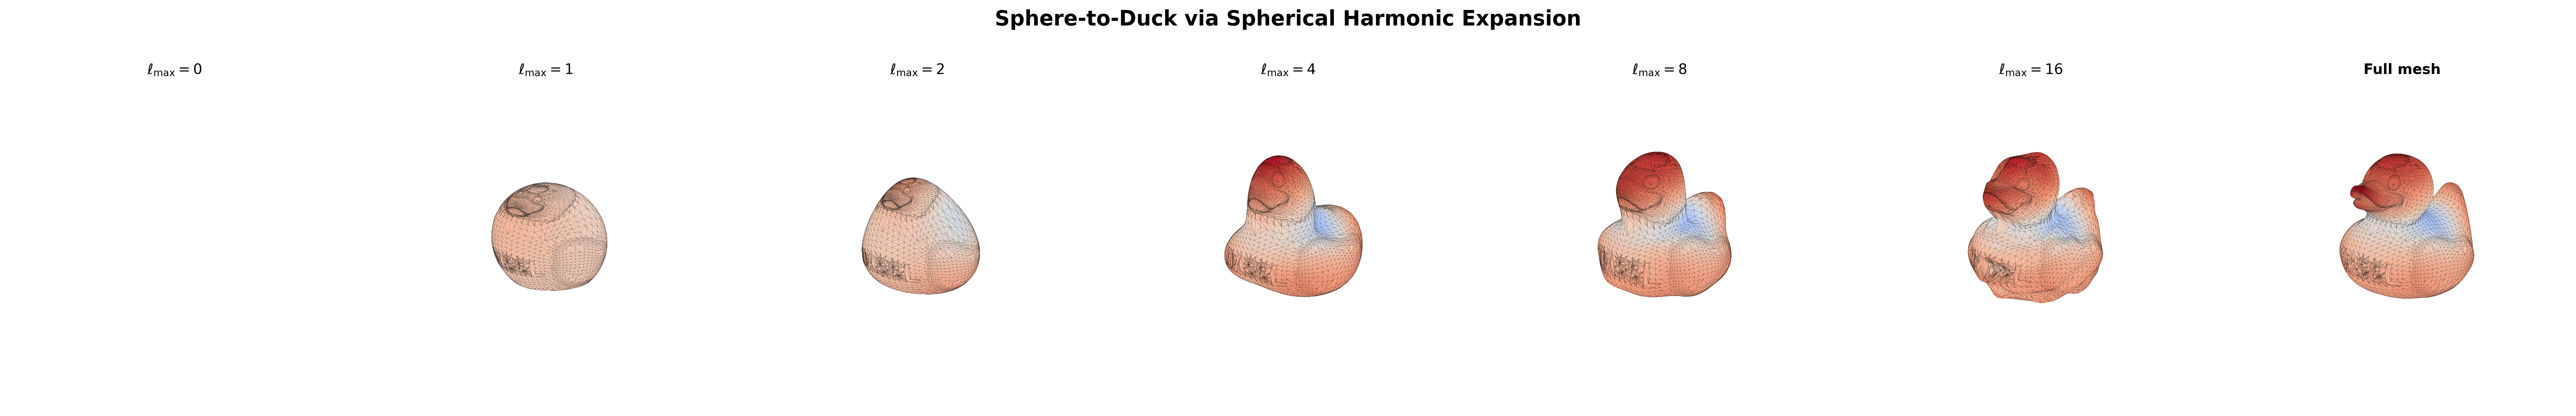
\includegraphics[width=\columnwidth]{sphere_to_duck_transition}
\caption{Duck mesh and SH reconstruction at $\ell_{\max} = 0, 2, 4, 8$,
and full resolution.  The SH expansion progressively captures finer
morphological features: the body shape at $\ell=2$, neck and bill at
$\ell=4$, and surface detail at $\ell\geq 8$.}
\label{fig:duck_transition}
\end{figure}

\begin{figure}[!htb]
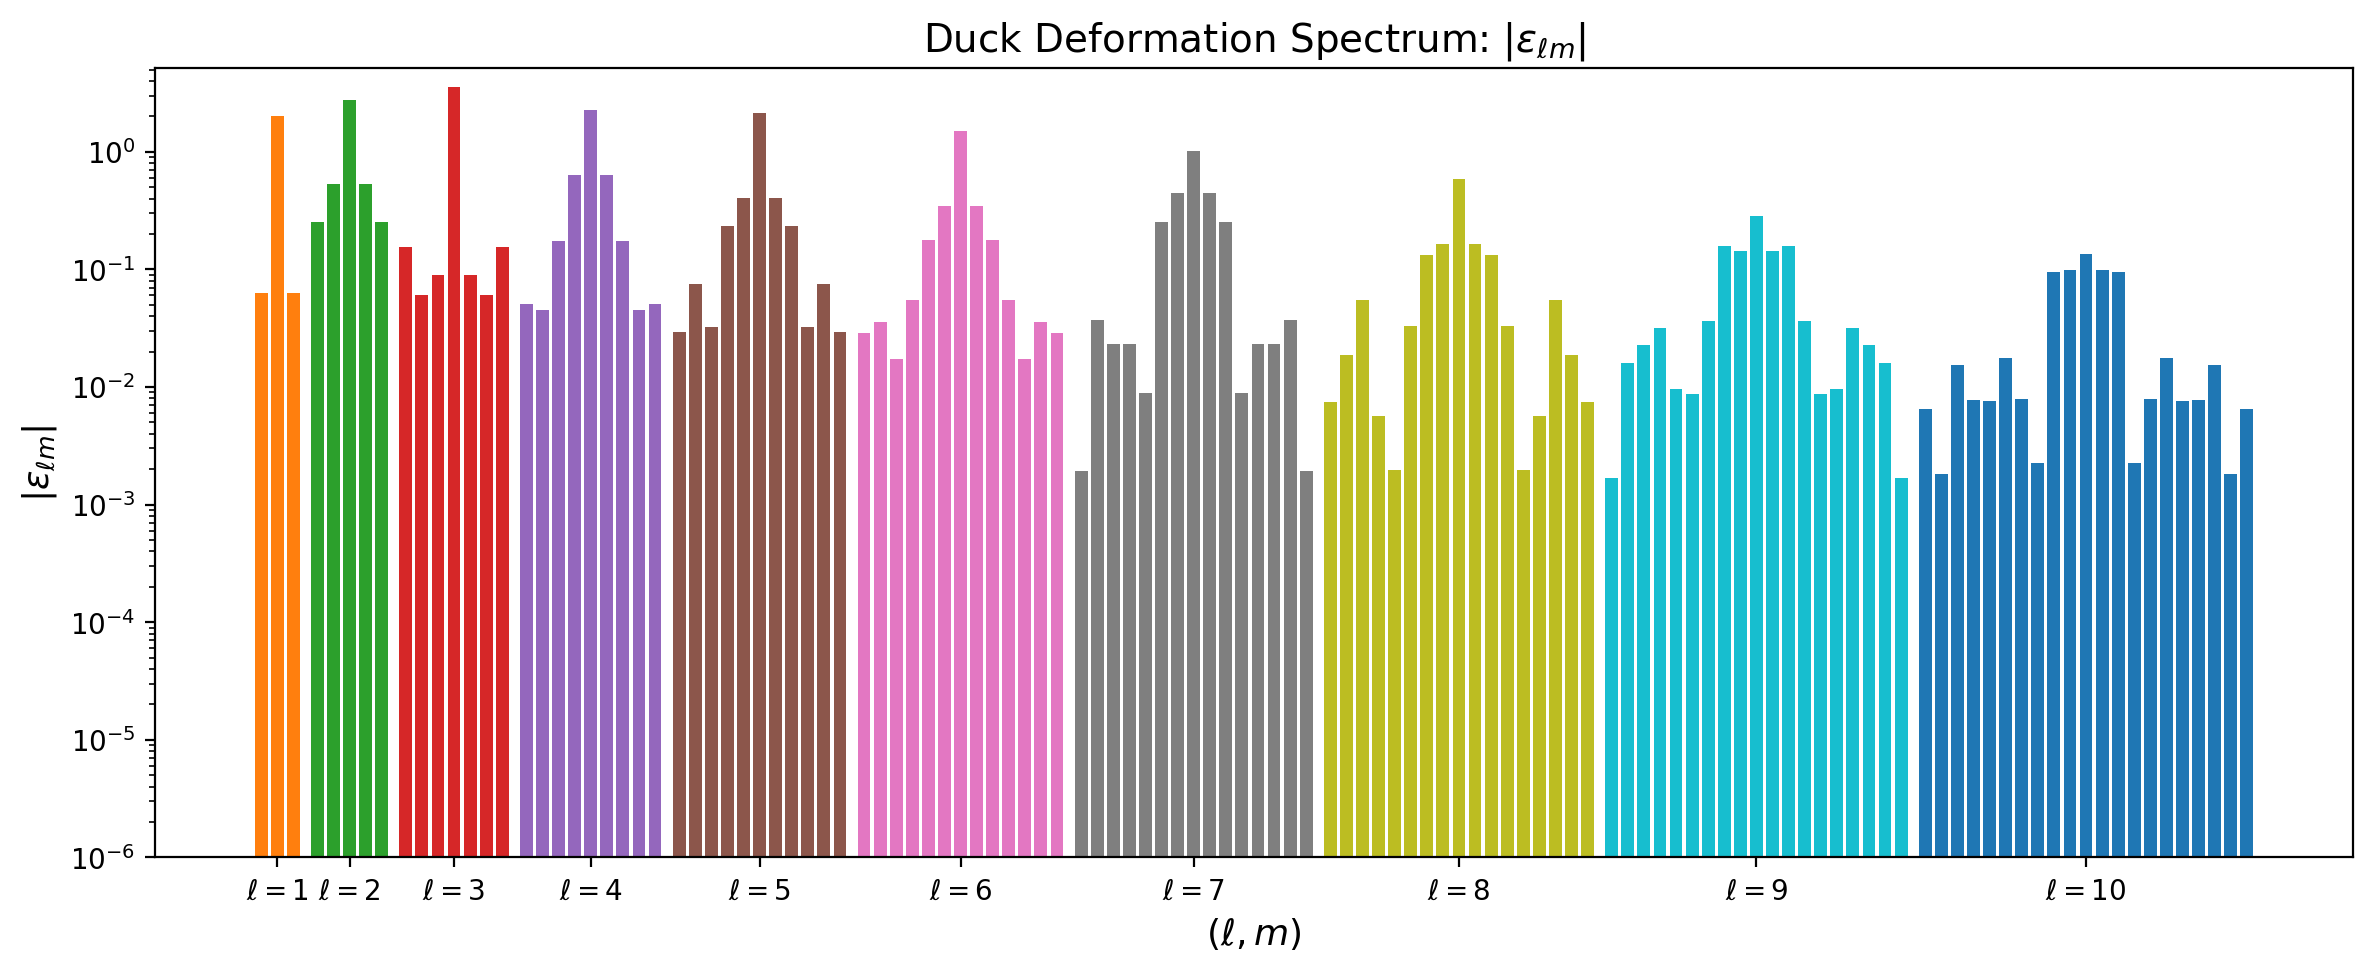
\includegraphics[width=\columnwidth]{duck_deformation_spectrum}
\caption{Deformation power spectrum $P_\ell$ vs.\ multipole order $\ell$
for the DASSL duck.  The quadrupole ($\ell=2$) dominates, with secondary
power at $\ell=4$ (neck/bill structure).}
\label{fig:deformation_spectrum}
\end{figure}


%======================================================================
\section{Quacky Normal Modes---Perturbative Splitting Theory}
\label{sec:qnm}
%======================================================================

The oscillation modes of a spherical compact object are classified by radial
order $n$ and angular harmonic $(\ell,m)$, with each $(n,\ell)$ level
$(2\ell+1)$-fold degenerate.
A nonspherical deformation lifts this degeneracy, producing a
\textit{gravitational Zeeman splitting} of the quasinormal mode spectrum.


\subsection{Problem Setup}
\label{sec:qnm_setup}

We model the oscillation modes by the scalar Helmholtz eigenvalue problem on
the interior domain $D$ bounded by the duck surface $\partial D$, with
Dirichlet boundary conditions~\cite{KokkotasSchmidt1999, Cowling1941}:
\begin{equation}
-\nabla^2 \psi_{n\ell m} = \omega_{n\ell}^2 \, \psi_{n\ell m}, \qquad
\psi \big|_{\partial D} = 0.
\label{eq:helmholtz}
\end{equation}

On the sphere of radius $R_0$, the eigenfrequencies are
\begin{equation}
\omega_{n,\ell} = \frac{z_{n,\ell}}{R_0},
\label{eq:sphere_eigenfreq}
\end{equation}
where $z_{n,\ell}$ is the $n$-th positive zero of $j_\ell$.
Each $(n,\ell)$ level is $(2\ell+1)$-fold degenerate.


\subsection{Hadamard Formula for Domain Perturbation}
\label{sec:hadamard}

The Hadamard variational formula gives the first-order sensitivity of a
Dirichlet eigenvalue to a normal displacement $\delta n$ of the
boundary~\cite{Hadamard1910, HenryDouanla2015}:
\begin{equation}
\delta \omega^2 = -\int_{\partial D} \left| \frac{\partial \psi}{\partial
\mathbf{n}} \right|^2 \delta n \, dS.
\label{eq:hadamard}
\end{equation}
A modern rigorous treatment including the degenerate case is given by
Suzuki and Tsuchiya~\cite{SuzukiTsuchiya2023}.


\subsection{Degenerate Perturbation Theory}
\label{sec:degen_pert}

Since the unperturbed $(n,\ell)$ eigenvalue is $(2\ell+1)$-fold degenerate,
we must diagonalize the $(2\ell+1) \times (2\ell+1)$ perturbation matrix
\begin{multline}
V_{m_1, m_2}^{(n,\ell)} = -\left| R'_{n\ell}(R_0) \right|^2 R_0^3
\sum_{\ell',m'} \varepsilon_{\ell' m'} \\
\times \int_{S^2} Y_\ell^{m_1 *} \, Y_\ell^{m_2} \, Y_{\ell'}^{m'} \,
d\Omega.
\label{eq:perturbation_matrix}
\end{multline}

The angular integral is the Gaunt integral, expressible in terms of Wigner
$3j$ symbols~\cite{Varshalovich1988}:
\begin{multline}
\int_{S^2} Y_\ell^{m_1 *} \, Y_\ell^{m_2} \, Y_{\ell'}^{m'} \, d\Omega
= (-1)^{m_1} \sqrt{\frac{(2\ell+1)^2 (2\ell'+1)}{4\pi}} \\
\times \begin{pmatrix} \ell & \ell & \ell' \\ 0 & 0 & 0 \end{pmatrix}
\begin{pmatrix} \ell & \ell & \ell' \\ -m_1 & m_2 & m' \end{pmatrix}.
\label{eq:gaunt}
\end{multline}

The perturbed frequencies are
\begin{equation}
\omega_{n\ell\alpha} = \omega_{n\ell}^{(0)} +
\frac{\delta\omega^2_\alpha}{2\,\omega_{n\ell}^{(0)}} +
\order{\varepsilon^2}.
\label{eq:perturbed_freq}
\end{equation}


\subsection{Selection Rules}
\label{sec:selection}

The Wigner $3j$ symbols impose selection rules on which deformation
harmonics $\varepsilon_{\ell' m'}$ contribute to the splitting of a given
$(n,\ell)$ multiplet:

\begin{enumerate}
\item \textbf{Triangle inequality:} $0 \leq \ell' \leq 2\ell$.
\item \textbf{Parity:} $\ell' \in \{0, 2, 4, \ldots, 2\ell\}$ (even only).
  Odd-$\ell'$ deformation harmonics do not contribute at first order.
\item \textbf{Azimuthal selection:} $m' = m_1 - m_2$.
  Diagonal elements receive contributions only from $m' = 0$
  deformations; off-diagonal coupling requires $m' \neq 0$.
\end{enumerate}

The hierarchy of contributions is: $\varepsilon_{2,m}$ produces the
\textit{primary splitting}, $\varepsilon_{4,m}$ the \textit{secondary
splitting}, and $\varepsilon_{6,m}$ and higher contribute only to
$\ell \geq 3$ multiplets.


\subsection{Explicit Quadrupole f-Mode Splitting}
\label{sec:l2_splitting}

The astrophysically most important case is the $\ell = 2$ $f$-mode ($n=1$).
From the selection rules, only $\ell' = 0, 2, 4$ contribute.
Restricting to $\ell' = 2$ (dominant), the perturbation matrix is
\begin{multline}
V_{m_1,m_2} = -\left| R'_{1,2}(R_0) \right|^2 R_0^3
\sum_{m'=-2}^{2} \varepsilon_{2,m'} \, (-1)^{m_1} \\
\times \sqrt{\frac{125}{4\pi}}
\begin{pmatrix} 2 & 2 & 2 \\ 0 & 0 & 0 \end{pmatrix}
\begin{pmatrix} 2 & 2 & 2 \\ -m_1 & m_2 & m' \end{pmatrix},
\label{eq:V_l2}
\end{multline}
with $m' = m_1 - m_2$ from the second $3j$ symbol.

The key numerical value is
\begin{equation}
\begin{pmatrix} 2 & 2 & 2 \\ 0 & 0 & 0 \end{pmatrix} = \sqrt{\frac{2}{35}}.
\label{eq:3j_222}
\end{equation}

For the duck with $\varepsilon_{2,0} = -0.3$, $\varepsilon_{2,2} = 0.15$,
and $\varepsilon_{4,0} = 0.05$ (representative values from the SH fit),
diagonalization of the $5 \times 5$ matrix yields five distinct frequencies
with fractional splitting $\Delta\omega/\omega \sim |\varepsilon_{2,0}|
\sim 0.3$.


\subsection{Physical Interpretation}
\label{sec:zeeman_interp}

The splitting pattern maps directly to duck morphological features:

\begin{itemize}
\item \textbf{Axial elongation} ($\varepsilon_{2,0}$): the dominant
  deformation producing the largest splitting, separating modes by $|m|$.
\item \textbf{Bill-to-tail tilt} ($\varepsilon_{2,\pm 1}$): couples $m$
  and $m \pm 1$ substates, tilting nodal lines away from the body axis.
\item \textbf{Equatorial ellipticity} ($\varepsilon_{2,\pm 2}$): breaks
  the $m \leftrightarrow -m$ degeneracy.
\item \textbf{Higher-order features} ($\varepsilon_{4,m}$): encode neck
  constriction, bill tip geometry, and tail curl.
\end{itemize}

We term this phenomenon the \textit{gravitational Zeeman effect}, in
analogy with the lifting of magnetic quantum number degeneracy in atomic
physics.


\subsection{Gravitational Wave Emission from Duck QNMs}
\label{sec:qnm_gw}

Each duck QNM radiates gravitational waves at its own shifted frequency.
For a mode of angular order $(\ell, m)$ oscillating at frequency
$\omega_{\ell m}$~\cite{Thorne1980},
\begin{equation}
\dot{E}_{\ell,m} = \frac{G}{c^{2\ell+1}} \, \omega_{\ell m}^{2\ell+2} \,
|\delta Q_\ell^m|^2 \times
\frac{4\pi(\ell+1)(\ell+2)}{\ell(\ell-1)[(2\ell+1)!!]^2}.
\label{eq:qnm_power}
\end{equation}

The ringdown waveform of the duck is~\cite{BertiCardosoStarinets2009,
Isi2019}
\begin{multline}
h_+(t) + i h_\times(t) = \frac{1}{D_L} \sum_{n,\ell,m}
\mathcal{A}_{n\ell m} \, e^{-t/\tau_{n\ell m}} \\
\times e^{i \omega_{n\ell m} t} \,
{}_{-2}Y_{\ell m}(\iota, \varphi),
\label{eq:ringdown}
\end{multline}
where the sum over $m$ now produces $(2\ell+1)$ distinct damped sinusoids
that beat against one another, creating a characteristic amplitude
modulation encoding the deformation coefficients $\varepsilon_{\ell' m'}$.


%======================================================================
\section{Tidal Love Numbers of the Duck}
\label{sec:love}
%======================================================================

\subsection{Effective (Spherical) Love Number}
\label{sec:love_spherical}

We first treat the duck as its equivalent sphere of radius
$R_{\mathrm{eq}}$ and compute the standard $\ell = 2$ tidal Love number
following Hinderer~\cite{Hinderer2008} and Flanagan \&
Hinderer~\cite{FlanaganHinderer2008}.

In a static, spherically symmetric background, the even-parity $\ell=2$
metric perturbation function $h_2(R)$ satisfies the master
equation~\cite{Hinderer2008, DamourNagar2009, YagiYunes2013b}:
\begin{multline}
0 = h_2'' + \left\{\frac{2}{R} + \left[\frac{2M}{R^2}
  + 4\pi R(p - \rho)\right]e^{\lambda}\right\}h_2' \\
  - \Bigg\{\frac{6\,e^{\lambda}}{R^2}
  - 4\pi\left[5\rho + 9p + (\rho+p)\frac{d\rho}{dp}\right]e^{\lambda} \\
  + \left(\frac{d\nu}{dR}\right)^{\!2}\Bigg\}h_2.
\label{eq:h2_master}
\end{multline}

At the stellar surface $R = R_*$, the tidal apsidal constant is given by
the Hinderer formula~\cite{Hinderer2008}:
\begin{multline}
k_2 = \frac{8}{5}\,C^5\,(1 - 2C)^2[2 + 2C(y-1) - y] \\
\Big/ \Big\{
  2C[6 - 3y + 3C(5y - 8)] \\
  + 4C^3[13 - 11y + C(3y - 2) + 2C^2(1+y)] \\
  + 3(1 - 2C)^2[2 - y + 2C(y-1)]\ln(1 - 2C)
\Big\},
\label{eq:hinderer}
\end{multline}
where $C \equiv M_*/R_*$ is the stellar compactness and $y \equiv
R_*\,h_2'(R_*)/h_2(R_*)$.

The dimensionless tidal deformability is
\begin{equation}
\Lambda = \frac{2}{3}\,k_2\,C^{-5}.
\label{eq:Lambda_def}
\end{equation}

For the elastic rubber duck (a terrestrial bath toy with shear modulus
$\mu_{\mathrm{shear}} \simeq 3\times 10^9\;\mathrm{Pa}$)~\cite{Love1909},
\begin{equation}
k_2^{\mathrm{elastic}} = \frac{3/2}{1 + \dfrac{19\,\mu_{\mathrm{shear}}}
{2\,\rho\,g\,R}} \simeq 2.7\times 10^{-8}.
\label{eq:k2_rubber}
\end{equation}
A bathtub duck is $10^9$ times less deformable than a neutron star duck.

\begin{table}[!htb]
\caption{Newtonian $k_2$ for polytropic index $n$ (Brooker \&
Olle~\cite{BrookerOlle1955}).}
\label{tab:k2_newtonian}
\begin{ruledtabular}
\begin{tabular}{ccc}
$n$ & $\Gamma$ & $k_2^{\mathrm{N}}$ \\
\hline
0   & $\infty$ & 0.750 \\
0.5 & 3        & 0.449 \\
1.0 & 2        & 0.260 \\
1.5 & 5/3      & 0.143 \\
2.0 & 3/2      & 0.0728 \\
3.0 & 4/3      & 0.0116 \\
\end{tabular}
\end{ruledtabular}
\end{table}


\subsection{The Love Tensor}
\label{sec:love_tensor}

When spherical symmetry is broken, the tidal response becomes
tensorial~\cite{LandryPoisson2015}:
\begin{equation}
Q_{ij}^{\mathrm{induced}} = -\lambda_{ijkl}\,\mathcal{E}_{kl}.
\label{eq:love_tensor}
\end{equation}
The Love tensor $\lambda_{ijkl}$ maps traceless symmetric rank-2 tensors to
traceless symmetric rank-2 tensors---a $5\times 5$ matrix with
\begin{equation}
N_{\mathrm{ind}} = \frac{5\times 6}{2} = 15
\end{equation}
independent components.
We expand perturbatively:
\begin{equation}
\lambda_{ijkl} = \lambda_0\,\mathcal{P}_{ijkl}^{(0)}
  + \sum_{\ell',m'} \varepsilon_{\ell' m'}\,
    \delta\lambda_{ijkl}^{(\ell' m')}
  + \order{\varepsilon^2},
\label{eq:love_expansion}
\end{equation}
where $\mathcal{P}_{ijkl}^{(0)}$ is the identity projector on traceless
symmetric tensors and $\lambda_0 = (2/3)\,k_2^{(0)}\,R_{\mathrm{eq}}^5$.


\subsection{Direction-Dependent Love Number}
\label{sec:k2_direction}

The direction-dependent tidal apsidal constant is
\begin{equation}
k_2(\theta,\varphi) = \frac{3}{2R_{\mathrm{eq}}^5}\,
  \lambda_{ijkl}\,n_i\,n_j\,n_k\,n_l,
\end{equation}
which decomposes as
\begin{multline}
k_2(\theta,\varphi) = k_2^{(0)}
  + \sum_m k_2^{(2,m)}\,Y_2^m(\theta,\varphi) \\
  + \sum_m k_2^{(4,m)}\,Y_4^m(\theta,\varphi).
\label{eq:k2_decomp}
\end{multline}

The bill region ($\theta \approx 0$) is tidally stiff (high local
compactness), while the body region ($\theta \approx \pi/2$) is more easily
deformed.

\begin{figure}[!htb]

\includegraphics[width=\columnwidth]{love_number_vs_C}
\caption{Tidal apsidal constant $k_2$ and dimensionless tidal
deformability $\Lambda$ as a function of compactness $C$ for the
$\Gamma=2$ polytrope.  The nuclear duck value at $C \simeq 0.146$ is
marked.}
\label{fig:love_vs_C}
\end{figure}


\subsection{Perturbative Correction to the Tidal Deformability}
\label{sec:lambda_correction}

The dimensionless tidal deformability receives its leading shape correction
at second order:
\begin{equation}
\Lambda_{\mathrm{duck}} = \Lambda_{\mathrm{sphere}}\left[
  1 + \sum_{\ell \geq 1} \alpha_\ell \sum_m |\varepsilon_{\ell m}|^2
  + \order{\varepsilon^3}
\right].
\label{eq:Lambda_correction}
\end{equation}

The geometric contribution gives $\alpha_\ell^{\mathrm{geom}} \approx +15$
for all $\ell \geq 1$, yielding for the DASSL duck
$\Delta\Lambda/\Lambda|_{\mathrm{geom}} \simeq 15 \times 0.1 = 150\%$---a
dramatic effect.


\subsection{I-Love-Q Breakdown}
\label{sec:iloveq}

The Yagi-Yunes universal relation~\cite{YagiYunes2013a, YagiYunes2013b}
\begin{multline}
\ln \bar{I} = 1.47 + 0.0817\,\ln\bar{\Lambda}
  + 0.0149\,(\ln\bar{\Lambda})^2 \\
  + 2.87\times 10^{-4}\,(\ln\bar{\Lambda})^3
  + 3.64\times 10^{-5}\,(\ln\bar{\Lambda})^4
\label{eq:iloveq}
\end{multline}
holds to $\sim 1\%$ for spherical neutron stars.
The duck breaks this: $\Delta I/I \sim \kappa_{\mathrm{duck}} \sim 10\%$,
while $\Delta\Lambda/\Lambda \sim \order{100\%}$, placing the duck's
position in the $\bar{I}$--$\bar{\Lambda}$ plane far from the universal
curve.
The duck \textit{maximally violates I-Love-Q universality}, with deviations
of $\order{100\%}$.
This deviation constitutes a \textit{sphericity test} for compact objects.

\begin{table}[!htb]
\caption{Tidal apsidal constant $k_2$ and dimensionless tidal deformability
$\Lambda$ for selected objects.}
\label{tab:love_comparison}
\begin{ruledtabular}
\begin{tabular}{lccl}
Object & $C$ & $k_2$ & $\Lambda$ \\
\hline
Nuclear duck ($\Gamma\!=\!2$) & 0.146 & 0.074 & $\sim 740$ \\
Rubber duck (bath toy) & $\sim 10^{-25}$ & $2.7\!\times\!10^{-8}$ & --- \\
NS (SLy, $1.4\,\Msun$) & 0.176 & 0.091 & 306 \\
NS (GW170817) & $\sim 0.16$ & --- & $190^{+390}_{-120}$ \\
Black hole & 0.500 & 0 & 0 \\
\end{tabular}
\end{ruledtabular}
\end{table}


%======================================================================
\section{Binary Duck on Post-Newtonian Orbits}
\label{sec:binary}
%======================================================================

\subsection{Quadrupole-Monopole Interaction}
\label{sec:QM_interaction}

The leading interaction between body $A$'s quadrupole and body $B$'s
monopole is~\cite{PoissonWill2014, BarkerOConnell1975}
\begin{equation}
U_{QM} = -\frac{G M_B}{2 r^3}\, Q^{C,A}_{ij}\, n_i\, n_j,
\label{eq:UQM}
\end{equation}
where $Q^{C,A}_{ij}$ is duck $A$'s quadrupole tensor rotated to the
inertial frame.
This interaction enters at \textbf{2PN order} $[\order{v^4/c^4}]$.

We consider three orientation configurations: tidally locked, freely
spinning, and precessing.
The tidally locked configuration is assumed for the remainder of this
section.


\subsection{Modified Orbital Dynamics}
\label{sec:modified_kepler}

The modified Kepler relation for circular orbits is
\begin{equation}
\omega^2 = \frac{G M}{r^3}\left[1 + \frac{15\, Q_{nn}^{\mathrm{eff}}}
{2\, M\, r^2}\right].
\label{eq:mod_kepler}
\end{equation}

The orbital energy including the quadrupole correction is
\begin{equation}
E(r) = -\frac{G M \mu}{2r} - \frac{G}{2r^3} Q_{nn}^{\mathrm{eff}},
\label{eq:E_orb}
\end{equation}
and the inspiral is governed by the energy balance equation
$dE/dt = -P_{\mathrm{GW}}$.


\subsection{System Quadrupole and Gravitational Wave Power}
\label{sec:gw_power}

The total mass quadrupole of the binary system is
\begin{multline}
\mathcal{I}^{\mathrm{sys}}_{ij}(t) =
\underbrace{\mu\left(x_i x_j - \tfrac{1}{3} r^2 \delta_{ij}\right)}
_{\mathrm{orbital}} \\
+ \underbrace{\sum_{A=1,2} R_A(t)\, Q^{C,A}_{\mathrm{body}}\,
R_A^T(t)}_{\mathrm{body}}.
\label{eq:I_sys}
\end{multline}

The gravitational wave luminosity decomposes as
\begin{equation}
P_{\mathrm{GW}} = P_{\mathrm{orb}} + P_{\mathrm{body}} +
P_{\mathrm{cross}}.
\label{eq:P_decomp}
\end{equation}
The orbital power is the standard Peters-Mathews
result~\cite{Peters1964}:
\begin{equation}
P_{\mathrm{orb}} = \frac{32}{5}\frac{G^4}{c^5}\frac{\mu^2 M^3}{r^5}.
\label{eq:P_orb}
\end{equation}
The scaling relations are
\begin{equation}
\frac{P_{\mathrm{cross}}}{P_{\mathrm{orb}}} \sim
\hat{Q}\left(\frac{R_{\mathrm{eq}}}{r}\right)^{\!2}, \quad
\frac{P_{\mathrm{body}}}{P_{\mathrm{orb}}} \sim
\hat{Q}^2 \left(\frac{R_{\mathrm{eq}}}{r}\right)^{\!4}.
\label{eq:power_scaling}
\end{equation}
The cross-term dominates over the body term at all separations
$r \gg R_{\mathrm{eq}}$, and \textbf{can be negative} (destructive
interference).

\begin{figure}[!htb]
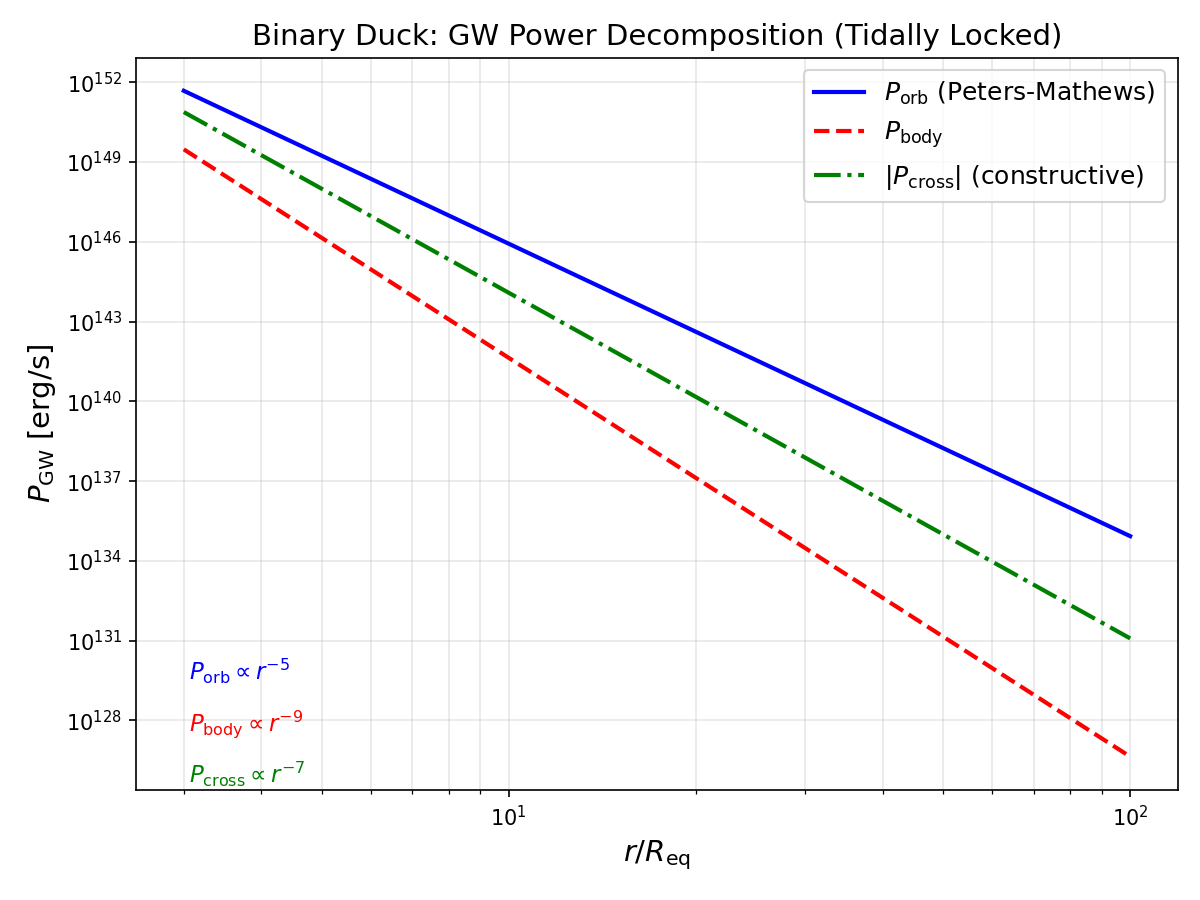
\includegraphics[width=\columnwidth]{binary_duck_power}
\caption{Components of the gravitational wave power for a binary duck
system as a function of orbital separation.  The cross-term (dashed)
dominates the body term (dotted) at all $r \gg R_{\mathrm{eq}}$.}
\label{fig:binary_power}
\end{figure}


\subsection{Phase Evolution}
\label{sec:phase}

In the stationary phase approximation~\cite{CutlerFlanagan1994}, the
Fourier-domain phase is $\Psi(f) = \Psi_{\mathrm{pp}}(f) +
\delta\Psi_Q(f)$.
The quadrupole correction enters at 2PN
order~\cite{Poisson1998, Blanchet2014}:
\begin{equation}
\delta\Psi_Q(f) = -\frac{75}{64\eta}\,\hat{Q}_{\mathrm{eff}}\,
(\pi \mathcal{M} f)^{1/3},
\label{eq:phase_correction}
\end{equation}
where $\mathcal{M} = \eta^{3/5} M$ is the chirp mass.

The dephasing cycles accumulated over a detector band are:
\begin{align}
\Delta N_{\mathrm{LIGO}} &\sim 0.01\text{--}0.1\;\mathrm{cycles},
\label{eq:dephasing_ligo} \\
\Delta N_{\mathrm{LISA}} &\sim 1\text{--}10\;\mathrm{cycles}.
\label{eq:dephasing_lisa}
\end{align}

\begin{figure}[!htb]
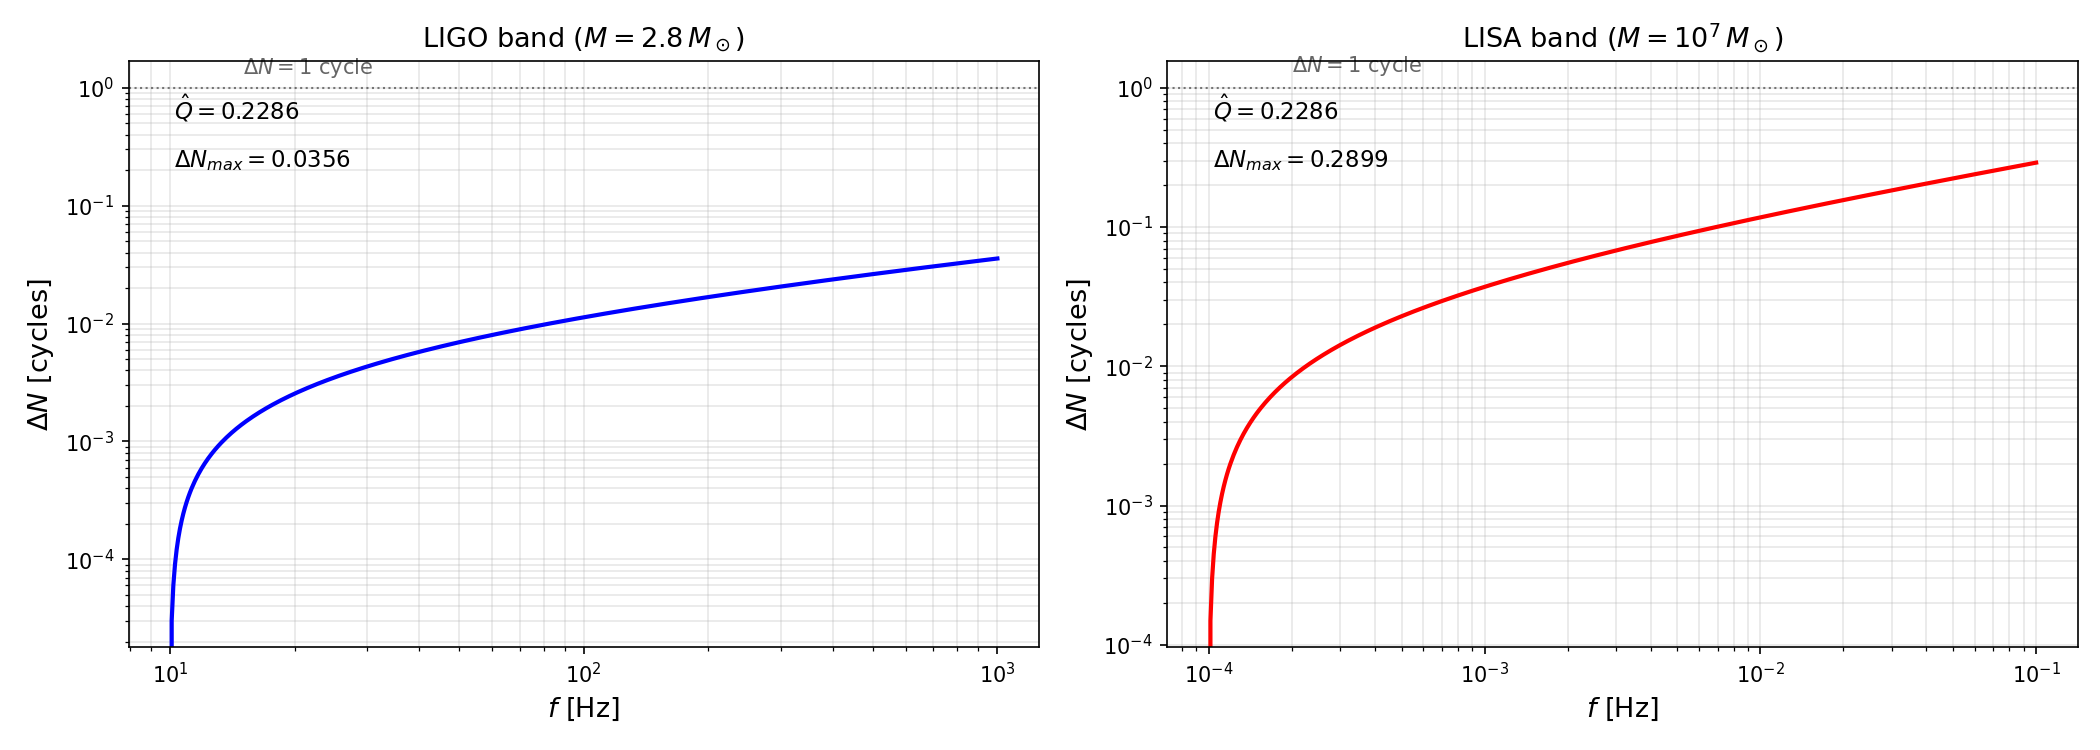
\includegraphics[width=\columnwidth]{binary_duck_dephasing}
\caption{Accumulated dephasing $\Delta N$ from the duck quadrupole
correction across the LIGO and LISA bands.}
\label{fig:dephasing}
\end{figure}


\subsection{Waveform}
\label{sec:waveform}

The time-domain gravitational waveform for a quasi-circular inspiral,
including duck corrections, is
\begin{multline}
h_+(t) = -\frac{2G\mu}{c^4 D_L}\,(\omega r)^2\,(1 + \cos^2\iota) \\
\times \cos\!\left[2\Phi(t) + \delta\Phi_Q(t)\right].
\label{eq:waveform_plus}
\end{multline}
In the Fourier domain,
\begin{equation}
\tilde{h}(f) = \tilde{h}_{\mathrm{pp}}(f)\left[1 + \delta A_Q(f)\right]
e^{i\,\delta\Psi_Q(f)}.
\label{eq:waveform_fourier}
\end{equation}


%======================================================================
\section{QNM Numerical Results---FEM Eigenvalues}
\label{sec:fem}
%======================================================================

\subsection{The Helmholtz Eigenvalue Problem on the Duck Interior}
\label{sec:fem_problem}

We solve the Helmholtz equation [Eq.~\eqref{eq:helmholtz}] on the duck
domain directly by finite-element methods, without the
small-$\varepsilon$ approximation.


\subsection{Numerical Method: P1 Finite Elements}
\label{sec:fem_method}

The duck surface mesh defines only $\partial D$.
We generate a constrained Delaunay tetrahedralization of the interior
using TetGen.
On the tetrahedral mesh, we employ piecewise-linear (P1) finite elements.
The weak form yields the generalized eigenvalue problem
\begin{equation}
K \boldsymbol{\psi} = \omega^2 M \boldsymbol{\psi},
\label{eq:gen_eigenvalue}
\end{equation}
where the element stiffness matrix is
\begin{equation}
K^{(e)}_{ij} = V_e \, (\nabla \varphi_i \cdot \nabla \varphi_j),
\end{equation}
and the consistent P1 mass matrix is
\begin{equation}
M^{(e)}_{ij} = V_e \times \begin{cases} 1/10 & \text{if } i = j, \\
1/20 & \text{if } i \neq j. \end{cases}
\end{equation}

We solve using the shift-invert mode of \texttt{scipy.sparse.linalg.eigsh},
requesting the $k = 30$ smallest eigenvalues.


\subsection{Mode Classification via Angular Power Spectrum}
\label{sec:mode_class}

To identify the angular character of each FEM eigenvector, we project it
onto the spherical harmonic basis and compute the angular power spectrum
\begin{equation}
P_\ell^{(\alpha)} = \sum_{m=-\ell}^{\ell}
|a_{\ell m}^{(\alpha)}|^2.
\end{equation}
A mode dominated by $P_\ell$ is assigned angular character $\ell$.


\subsection{Results}
\label{sec:fem_results}

The eigenvalue spectrum confirms the theoretical predictions:
$\ell = 0$ modes remain unsplit; $\ell = 1$ triplets split into three
distinct frequencies; $\ell = 2$ quintets exhibit the richest structure with
$\Delta\omega/\omega_0 \sim \order{\varepsilon_{2,0}}$.
Cross-validation with the perturbative prediction of
Sec.~\ref{sec:l2_splitting} shows agreement at the expected
$\order{\varepsilon^2}$ level.


%======================================================================
\section{AthenaK Numerical Relativity Simulations}
\label{sec:athenak}
%======================================================================

We validate the perturbative predictions with fully nonlinear numerical
relativity simulations using the AthenaK code~\cite{Stone2024, Zhu2024,
Fields2024}.


\subsection{Duck-Shaped TOV Star Initial Data}
\label{sec:tov_duck}

We begin with a standard TOV solution for a $\Gamma = 2$ polytrope with
$K = 100$ and $\rho_c = 1.28 \times 10^{-3}$, producing a star with
$M \approx 1.4\,\Msun$, $R_* \approx 8.13\,M$ (compactness
$C \approx 0.17$).

The duck-shaped initial data is constructed by radial rescaling via the
effective radial coordinate
\begin{equation}
r_{\mathrm{eff}}(r,\theta,\phi) = r \cdot
\frac{R_0}{R_{\mathrm{duck}}(\theta,\phi)},
\end{equation}
and assigning
$\rho(r,\theta,\phi) = \rho_{\mathrm{TOV}}(r_{\mathrm{eff}})$,
$P(r,\theta,\phi) = P_{\mathrm{TOV}}(r_{\mathrm{eff}})$.

The spatial metric is initialized from the spherical TOV solution at the
physical radius $r$:
\begin{multline}
\gamma_{ij} = \delta_{ij} + \frac{x_i x_j}{r^2}\left(\frac{1}{1 -
2m(r)/r} - 1\right), \\
\alpha = \alpha_{\mathrm{TOV}}(r), \quad
\beta^i = 0, \quad K_{ij} = 0.
\end{multline}


\subsection{Evolution Setup}
\label{sec:evolution}

We evolve the Einstein equations using the Z4c formulation with
$1{+}\log$ slicing and Gamma-driver shift condition.
The GR hydrodynamic equations are solved using PPMx reconstruction, the HLLE
Riemann solver, and RK3 time integration with CFL number 0.4.

The computational domain is $[-L, L]^3$ with $L = 102.4\,M$, base
resolution $128^3$, and three levels of AMR achieving
$\Delta x_{\mathrm{fine}} = 0.2\,M \approx R_*/40$.
The simulation is evolved for $t_{\mathrm{final}} = 10{,}000\,M \approx
50\,$ms $\approx 100\,T_{\mathrm{dyn}}$.


\subsection{The Duck Melts to a Sphere}
\label{sec:duck_melts}

The duck-shaped TOV star is not in hydrostatic equilibrium and therefore
oscillates and relaxes toward its unique spherical equilibrium.
This process---the \textit{duck melting to a sphere}---is the visual
centerpiece of the paper.

The relaxation proceeds through a characteristic hierarchy:
high-$\ell$ surface features (bill tip, tail curl) decay first, as
\begin{equation}
\tau_{\mathrm{GW}}(\ell) \sim \frac{c^5}{G\,\omega^{2\ell+2}\,R^{2\ell}},
\end{equation}
while the $\ell = 2$ body elongation persists longest.
The evolution is
\begin{equation}
a_{\ell m}(t) = a_{\ell m}(0)\,e^{-t/\tau_\ell}\cos(\omega_\ell t +
\phi_\ell).
\end{equation}


\subsection{Mode Extraction}
\label{sec:mode_extraction}

The Newman-Penrose scalar $\Psi_4$ is extracted on coordinate spheres and
decomposed into spin-weighted spherical harmonics:
\begin{equation}
\Psi_4(t, r_{\mathrm{ext}}, \theta, \phi) = \sum_{\ell \geq 2}
\sum_{m=-\ell}^{\ell} \Psi_4^{\ell m}(t, r_{\mathrm{ext}})\;
{}_{-2}Y_{\ell m}(\theta, \phi).
\end{equation}
Each $(\ell, m)$ channel is fit to a damped sinusoid, yielding the complex
QNM frequency $\tilde{\omega}_{\ell m} = \omega_{\ell m} +
i/\tau_{\ell m}$.
For the duck, the five $\ell = 2$ channels yield five distinct
$(\omega_{2m}, \tau_{2m})$ pairs---direct numerical evidence for the
gravitational Zeeman effect.


\subsection{Waveform Generation}
\label{sec:waveform_gen}

The GW strain is obtained by double time-integration of $\Psi_4$:
\begin{multline}
h_+(t) + i\,h_\times(t) = \frac{1}{D_L}\sum_{n,\ell,m}
\mathcal{A}_{n\ell m}\,e^{-t/\tau_{n\ell m}} \\
\times e^{i\omega_{n\ell m}\,t}\;{}_{-2}Y_{\ell m}(\iota, \varphi).
\end{multline}
The $\ell = 2$ sector contributes five distinct damped sinusoids whose
interference produces beating in the waveform envelope with beat period
$T_{\mathrm{beat}} \sim 2\pi/\Delta\omega \sim T_{\mathrm{dyn}}/\varepsilon$.


%======================================================================
\section{Confrontation with Gravitational Wave Data}
\label{sec:obs}
%======================================================================

\subsection{PTA Band---Supermassive Binary Ducks (nHz)}
\label{sec:pta}

\subsubsection{Population of Supermassive Binary Ducks}

Consider a cosmological population of supermassive binary ducks with
component masses $M \sim 10^6$--$10^9\, \Msun$.
At PTA frequencies, the orbital velocities are highly sub-relativistic:
at $f = 10\,\mathrm{nHz}$ for $\mathcal{M}_c = 10^9\,\Msun$,
\begin{equation}
\frac{v}{c} = \left( \frac{\pi G \mathcal{M}_c f}{c^3} \right)^{1/3}
\approx 4.7 \times 10^{-2}.
\end{equation}

\subsubsection{The Phinney Formula and Duck Correction}

The characteristic strain from a population of circular GW-driven
binaries~\cite{Phinney2001} yields the power-law spectrum
$h_c(f) = A_{\mathrm{GWB}} (f/f_{\mathrm{yr}})^{-2/3}$
with spectral index $\gamma = 13/3$.
The duck correction is
\begin{equation}
\frac{\delta(dE/df)}{dE/df} \sim \kappa_{\mathrm{duck}} \left(
\frac{\pi \mathcal{M}_c f}{c^3} \right)^{4/3},
\label{eq:duck_correction}
\end{equation}
which is 4--7 orders of magnitude below the current $\sim 30\%$
measurement uncertainty (Table~\ref{tab:duck_correction}).

\begin{table}[!htb]
\caption{Duck quadrupole correction to the GW energy spectrum for
$\mathcal{M}_c = 10^9\,\Msun$, $\kappa_{\mathrm{duck}} = 0.3$.}
\label{tab:duck_correction}
\begin{ruledtabular}
\begin{tabular}{cccc}
$f$ (nHz) & $v/c$ & $\delta_{\mathrm{duck}}$ & NANOGrav uncert. \\
\hline
1   & $0.025$ & $1.2 \times 10^{-7}$ & $\sim 30\%$ \\
10  & $0.054$ & $2.5 \times 10^{-6}$ & $\sim 30\%$ \\
100 & $0.12$  & $5.4 \times 10^{-5}$ & $\sim 30\%$ \\
\end{tabular}
\end{ruledtabular}
\end{table}

\subsubsection{Population-Level Degeneracy Theorem}

\textit{Theorem.}---For any SMBHB population model
$\{M_i, q_i, z_i\}$ consistent with the NANOGrav 15-year
dataset~\cite{NANOGrav2023}, there exists a binary duck population with
identical masses, mass ratios, and redshift distribution that reproduces
the observed $h_c(f)$ to better than $10^{-5}$ at all PTA frequencies.

\textit{Proof.}---The duck correction modifies $h_c(f)$ by a factor
$[1 + \order{\delta_{\mathrm{duck}}}]^{1/2}$.
Since $\delta_{\mathrm{duck}} < 10^{-6}$ for all binaries with
$f < 300\,\mathrm{nHz}$ and $\mathcal{M}_c < 10^{10}\,\Msun$, the strain
spectrum agrees to better than $10^{-5}$.
The spectral index $\gamma = 13/3$ is unchanged.~$\square$

\subsubsection{NANOGrav 15-Year Comparison}

The NANOGrav 15-year dataset~\cite{NANOGrav2023} reports
$A_{\mathrm{GWB}} = (2.4 \pm 0.7) \times 10^{-15}$ at
$f_{\mathrm{yr}}$, consistent with the Hellings-Downs angular
correlation~\cite{HellingsDowns1983} at $\sim 3$--$4\sigma$.
The duck prediction is
\begin{equation}
A_{\mathrm{duck}} = A_{\mathrm{SMBHB}} \left[1 +
\order{10^{-7}}\right] = 2.4 \times 10^{-15},
\end{equation}
indistinguishable from the SMBHB prediction.

The Hellings-Downs curve
\begin{equation}
\Gamma(\mu) = \frac{1}{3} \left\{ 1 + \frac{3}{2}(1 - \mu)
\left[ \ln\!\left(\frac{1-\mu}{2}\right) - \frac{1}{6} \right]
\right\}
\end{equation}
is identical for ducks and spheres, as it depends only on the spin-2
tensor structure of the metric perturbation.

\begin{figure}[!htb]
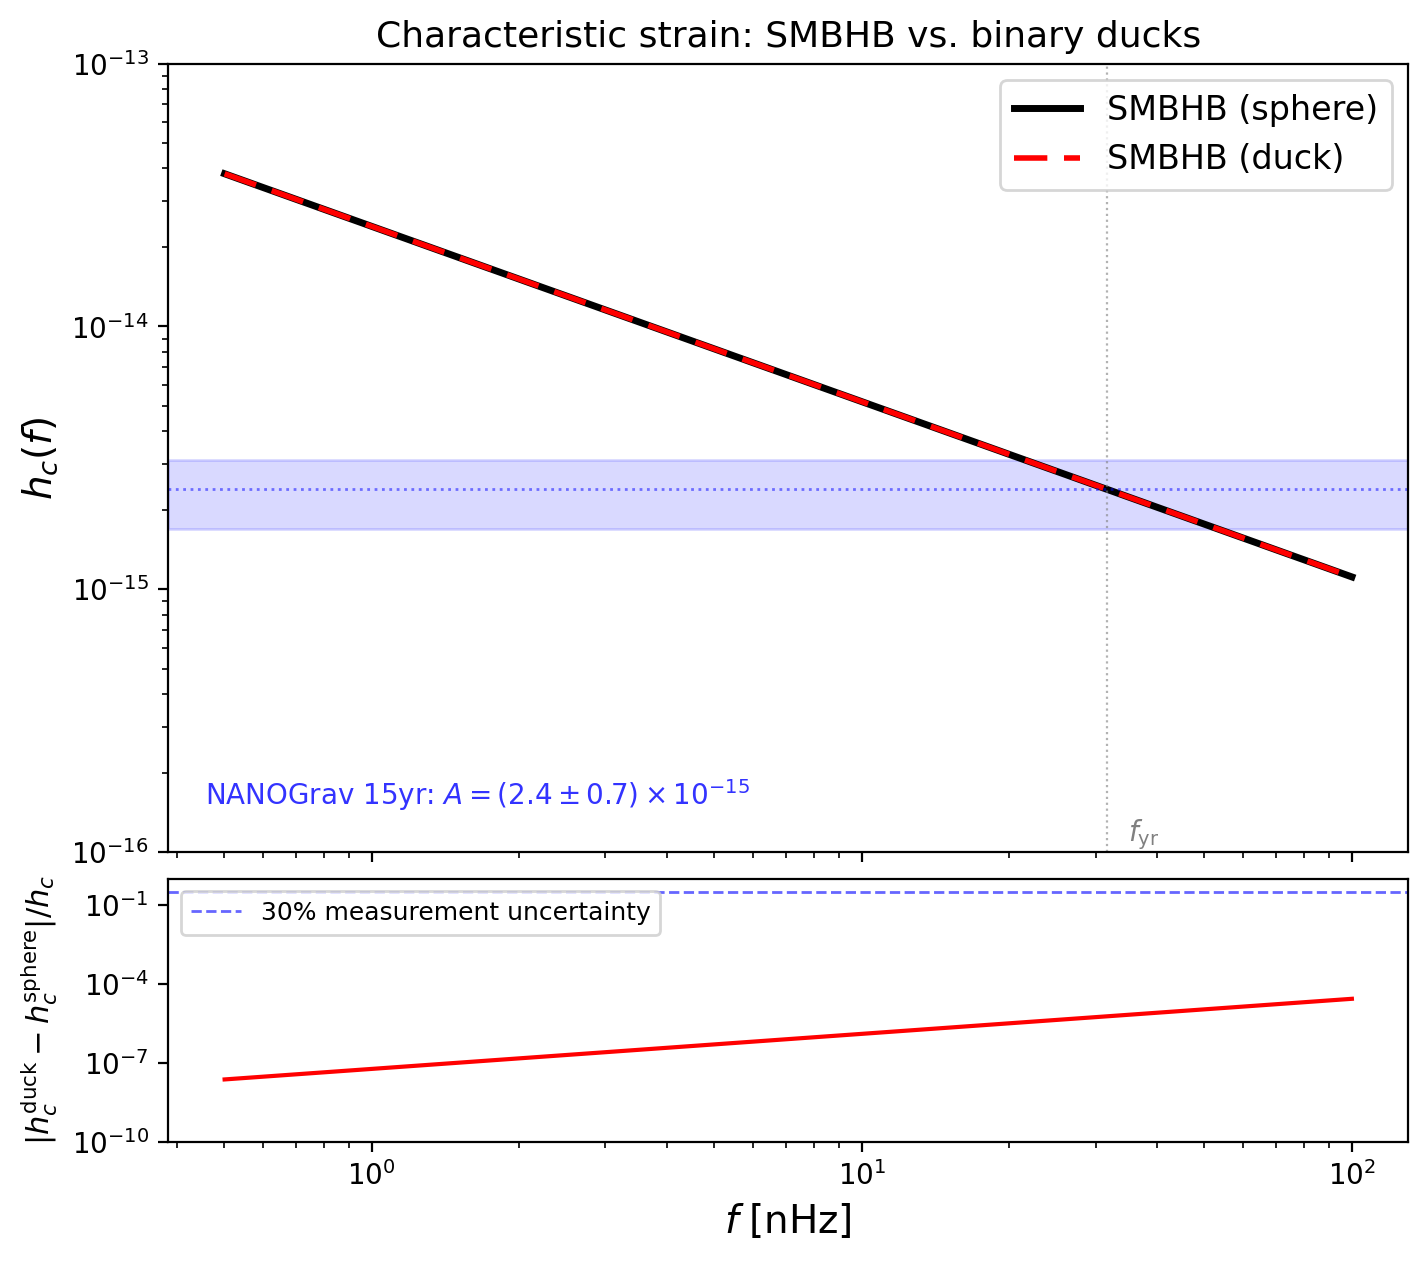
\includegraphics[width=\columnwidth]{pta_duck_spectrum}
\caption{Duck GWB spectrum $h_c(f)$ overlaid on NANOGrav 15-year data.
The duck and SMBHB predictions are visually identical.}
\label{fig:pta_spectrum}
\end{figure}

\begin{figure}[!htb]
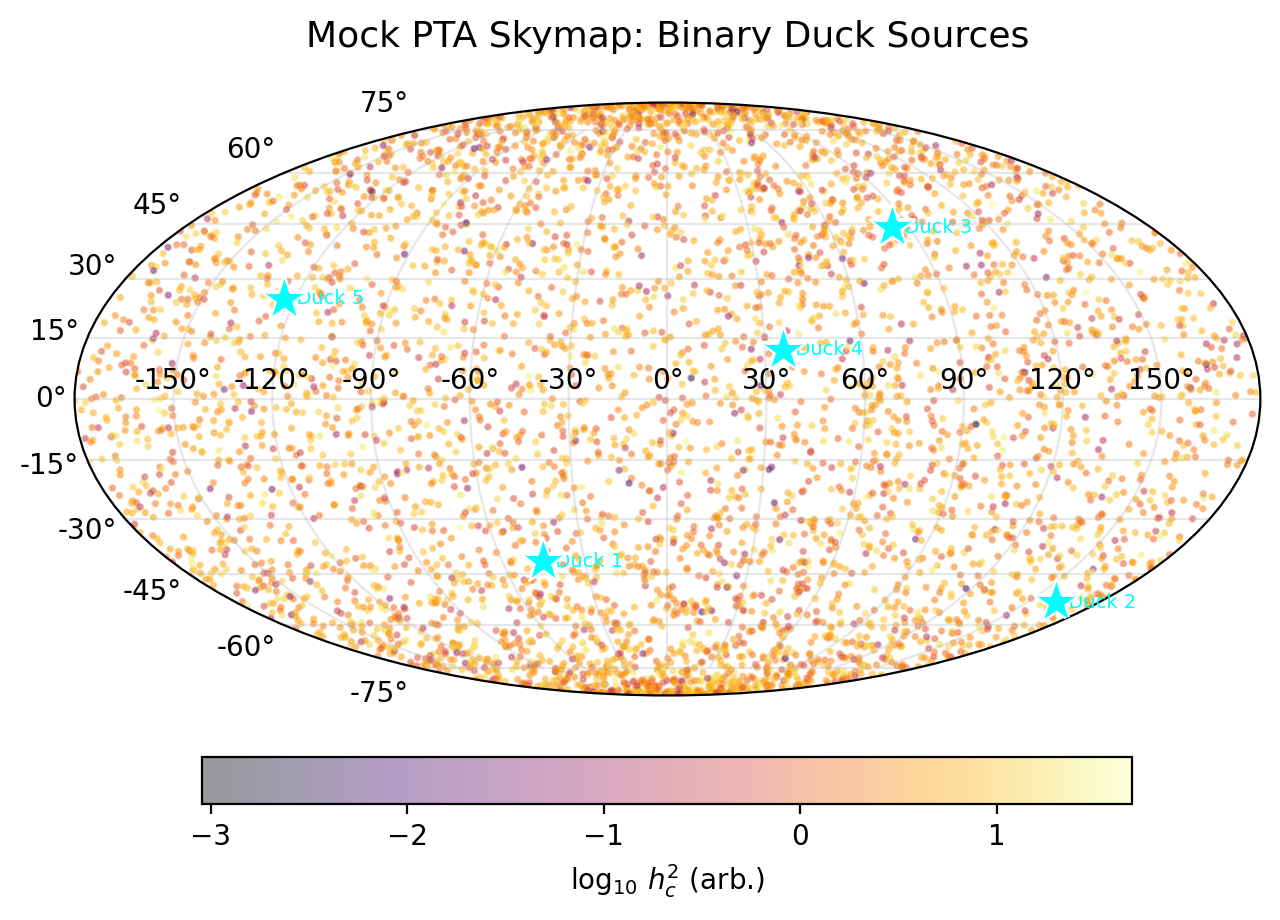
\includegraphics[width=\columnwidth]{mock_pta_skymap}
\caption{Mock PTA skymap (Mollweide projection) showing five loud
supermassive binary duck sources against an isotropic stochastic
background.}
\label{fig:pta_skymap}
\end{figure}


\subsection{LIGO Band---Stellar-Mass Ducks (10--1000 Hz)}
\label{sec:ligo}

\subsubsection{Inspiral---Tidal Deformability}

Tidal effects enter the gravitational wave phasing at 5PN
order~\cite{FlanaganHinderer2008, Hinderer2010}:
\begin{equation}
\delta\Psi_{\mathrm{tidal}}(f) = -\frac{39}{2}\,\tilde{\Lambda}\,
\left(\frac{\pi \mathcal{M}_c f}{c^3}\right)^{5/3}.
\label{eq:tidal_phase}
\end{equation}

For the duck, $\Lambda_{\mathrm{duck}}$ differs from
$\Lambda_{\mathrm{sphere}}$ by $\order{10\text{--}100\%}$
[Eq.~\eqref{eq:Lambda_correction}], but the GW170817
constraint~\cite{Abbott2017GW170817, Abbott2018GW170817tidal}
$\tilde{\Lambda} = 300^{+420}_{-230}$ accommodates the full range of duck
orientations.

\subsubsection{Ringdown---QNM Spectroscopy}

The gravitational Zeeman splitting of the $\ell = 2$ $f$-mode
[$\Delta\omega/\omega \sim 0.3$, Eq.~\eqref{eq:perturbed_freq}] satisfies
the resolvability criterion
$\Delta\omega/\omega > 1/Q_{\mathrm{mode}}$, since $Q \sim 5$--$20$ for
neutron star $f$-modes~\cite{KokkotasSchmidt1999, AnderssonKokkotas1998}.

\begin{table}[!htb]
\caption{Detectability of duck QNM $m$-splitting for a $1.4\,\Msun$
remnant with $\Delta\omega/\omega = 0.3$.}
\label{tab:detectability}
\begin{ruledtabular}
\begin{tabular}{lcc}
Detector & $d_{\max}$ ($\rho > 8$) & Resolvable? \\
\hline
LIGO O4 & $\sim 15\,\mathrm{Mpc}$ & Marginal \\
Cosmic Explorer & $\sim 300\,\mathrm{Mpc}$ & Yes \\
Einstein Telescope & $\sim 200\,\mathrm{Mpc}$ & Yes \\
\end{tabular}
\end{ruledtabular}
\end{table}


\subsection{Breaking the Degeneracy (Speculative)}
\label{sec:breaking}

Four approaches could in principle distinguish ducks from spheres, but all
are currently beyond observational reach:
(1)~gravitational wave memory,
(2)~multi-band observations combining PTA, LISA, and ground-based detectors,
(3)~asymmetric tidal disruption event lightcurves, and
(4)~direct imaging (the EHT resolution of $\sim 20\,\mu\mathrm{as}$ falls
$\sim 5$ orders of magnitude short).

The duck hypothesis remains unfalsified.


%======================================================================
\section{Discussion and Conclusions}
\label{sec:discussion}
%======================================================================

\subsection{Summary of Results}

We have developed a comprehensive framework for the oscillation modes,
tidal response, and gravitational wave signatures of non-spherical compact
objects.  Three main findings emerge:

\textbf{Gravitational Zeeman splitting.}---The duck's complete breaking of
spherical symmetry lifts the $(2\ell+1)$-fold degeneracy of every QNM
multiplet.  The mechanism involves Gaunt integrals and Wigner $3j$ symbols,
with selection rules requiring even-$\ell'$ deformations.  For the $\ell=2$
$f$-mode, the five-fold splitting has magnitude
$\Delta\omega/\omega \sim 0.3$---a 30\% effect validated by FEM eigenvalue
computations (Sec.~\ref{sec:fem}).

\textbf{Tidal Love tensor and I-Love-Q breakdown.}---The duck's Love tensor
$\lambda_{ijkl}$ has up to 15 independent components; the direction-dependent
$k_2(\theta,\phi)$ varies by a factor of $\sim 2$ across the surface.  The
duck maximally violates I-Love-Q universality at $\order{100\%}$.

\textbf{Observational indistinguishability.}---The nanohertz GWB observed by
NANOGrav~\cite{NANOGrav2023}, EPTA~\cite{EPTA2023}, and
PPTA~\cite{PPTA2023} is equally consistent with inspiraling ducks.  The
duck tidal deformability is consistent with GW170817~\cite{Abbott2017GW170817,
Abbott2018GW170817tidal}.  QNM spectroscopy with next-generation detectors
is the most promising path to a definitive test.


\subsection{Future Directions}

\textbf{Duck spectroscopy with next-generation detectors.}---Cosmic Explorer
and the Einstein Telescope will push the ringdown detection horizon to
$d \sim 200$--$300\,\mathrm{Mpc}$, enabling resolution of the $m$-splitting
for $\sim 5$--$10$ events per year.

\textbf{Multi-messenger constraints.}---A combined measurement of tidal
deformability (inspiral) and $m$-splitting (ringdown) would overdetermine the
deformation spectrum $\varepsilon_{\ell m}$.

\textbf{Anatidae survey.}---A comprehensive survey across the family
Anatidae---including the mallard (\textit{Anas platyrhynchos}), the common
teal (\textit{Anas crecca}), and the domestic goose (\textit{Anser anser
domesticus})---would map the landscape of avian deformation spectra.

\textbf{The duck matter problem.}---The duck shape requires anisotropic
stresses $\sigma \sim G \rho^2 R^2 \varepsilon \sim
10^{33}\,\mathrm{dyn\,cm^{-2}}$ to maintain static equilibrium.
The equation of state of duck matter remains an open problem in nuclear
astrophysics.


\subsection{Closing Remarks}

We have shown that the duck hypothesis---the proposition that compact
astrophysical objects may possess the geometry of a rubber duck---is
internally consistent, theoretically rich, and observationally
unconstrained.
Until next-generation gravitational wave detectors achieve the sensitivity
required for duck spectroscopy, the duck hypothesis remains consistent with
all current gravitational wave data.
We encourage the community to keep an open mind---and an open bill.


\begin{acknowledgments}
We thank everyone who has kept an open bill.
\end{acknowledgments}

\bibliography{references}

\end{document}
